\documentclass{article}

%% This template is pieces of templates provided by Chi-Kit Lam for
%% CS395T in S2016, bits taken from
%% https://github.com/nykh/latex-shorthands/blob/master/myshorthands.tex, and
%% other configs scrapped together over time.

\PassOptionsToPackage{svgnames}{xcolor}
\usepackage[margin=1in]{geometry}
\usepackage{float,graphicx,tabularx}
\usepackage[labelformat=simple]{subcaption}
\usepackage{eqparbox}
\usepackage{amsmath,amsthm,amsfonts,amssymb}
\usepackage{bbm}
\usepackage{leftidx}
\usepackage{mathtools}
\usepackage{semantic}
\usepackage[version=4]{mhchem} % chemical formulae
\usepackage{hyperref}
\usepackage{parskip}  %Extra space on new paragraph, no indent
\usepackage{graphicx} 
\usepackage{natbib}

\renewcommand\thesubfigure{(\alph{subfigure})}

%%% Section Separators

\newcommand{\starhsep}{
\begin{center} 
  $\ast$~$\ast$~$\ast$
\end{center}}

\newcommand{\clubhsep}{
\begin{center} 
  $\clubsuit$~$\clubsuit$~$\clubsuit$
\end{center}}

%% Paired delimiters, use with \delim{*expression*}
\DeclarePairedDelimiter\abkt{\langle}{\rangle}
\DeclarePairedDelimiter\cbkt{\lbrace}{\rbrace}
\DeclarePairedDelimiter\rbkt{\lparen}{\rparen}
\DeclarePairedDelimiter\sbkt{\lbrack}{\rbrack}
\DeclarePairedDelimiter\abs{\lvert}{\rvert}
\DeclarePairedDelimiter\norm{\lVert}{\rVert}
\DeclarePairedDelimiter\floor{\lfloor}{\rfloor}
\DeclarePairedDelimiter\ceiling{\lceil}{\rceil}
\DeclarePairedDelimiterX\set[2]{\lbrack}{\rbrack}{#1 \colon #2}

%% Operators

\newcommand{\clapover}[2]{\overbrace{#1}_{\mathclap{#2}}}
\newcommand{\clapunder}[2]{\underbrace{#1}_{\mathclap{#2}}}

\DeclareMathOperator*{\argmin}{arg\,min}
\DeclareMathOperator*{\argmax}{arg\,max}
\DeclareMathOperator{\supp}{supp}
\newcommand{\defeq}{\stackrel{\text{def}}=}

\DeclareMathOperator{\matrixtranspose}{T}
\newcommand{\T}{{\matrixtranspose}}
\DeclareMathOperator{\frobeniusnorm}{F}
\newcommand{\Fro}{{\frobeniusnorm}}
\DeclareMathOperator{\diag}{diag}

\DeclareMathOperator*{\E}{E}
\DeclareMathOperator*{\Var}{Var}
\DeclareMathOperator*{\Cov}{Cov}
\DeclareMathOperator*{\Corr}{Corr}
\DeclareMathOperator{\BinDist}{Bin}
\DeclareMathOperator{\GaussDist}{N}
\DeclareMathOperator{\PoisDist}{Pois}
\DeclareMathOperator{\UnifDist}{U}
\DeclareMathOperator{\erf}{erf} % error function.

\DeclareMathOperator{\df}{d} % Differential form.
\DeclareMathOperator{\round}{\partial}

\DeclareMathOperator{\area}{area}
\DeclareMathOperator{\vol}{vol}

%% Variables. This may seem excessive but trust me it's quite nice

\newcommand{\eps}{\varepsilon}
\newcommand{\haat}{\widehat}

\newcommand{\bbA}{{\mathbb{A}}}
\newcommand{\bbB}{{\mathbb{B}}}
\newcommand{\bbC}{{\mathbb{C}}}
\newcommand{\bbD}{{\mathbb{D}}}
\newcommand{\bbE}{{\mathbb{E}}}
\newcommand{\bbF}{{\mathbb{F}}}
\newcommand{\bbG}{{\mathbb{G}}}
\newcommand{\bbH}{{\mathbb{H}}}
\newcommand{\bbI}{{\mathbb{I}}}
\newcommand{\bbJ}{{\mathbb{J}}}
\newcommand{\bbK}{{\mathbb{K}}}
\newcommand{\bbL}{{\mathbb{L}}}
\newcommand{\bbM}{{\mathbb{M}}}
\newcommand{\bbN}{{\mathbb{N}}}
\newcommand{\bbO}{{\mathbb{O}}}
\newcommand{\bbP}{{\mathbb{P}}}
\newcommand{\bbQ}{{\mathbb{Q}}}
\newcommand{\bbR}{{\mathbb{R}}}
\newcommand{\bbS}{{\mathbb{S}}}
\newcommand{\bbT}{{\mathbb{T}}}
\newcommand{\bbU}{{\mathbb{U}}}
\newcommand{\bbV}{{\mathbb{V}}}
\newcommand{\bbW}{{\mathbb{W}}}
\newcommand{\bbX}{{\mathbb{X}}}
\newcommand{\bbY}{{\mathbb{Y}}}
\newcommand{\bbZ}{{\mathbb{Z}}}
\newcommand{\bbone}{{\mathbbm{1}}}

\newcommand{\bfA}{{\mathbf{A}}}
\newcommand{\bfB}{{\mathbf{B}}}
\newcommand{\bfC}{{\mathbf{C}}}
\newcommand{\bfD}{{\mathbf{D}}}
\newcommand{\bfE}{{\mathbf{E}}}
\newcommand{\bfF}{{\mathbf{F}}}
\newcommand{\bfG}{{\mathbf{G}}}
\newcommand{\bfH}{{\mathbf{H}}}
\newcommand{\bfI}{{\mathbf{I}}}
\newcommand{\bfJ}{{\mathbf{J}}}
\newcommand{\bfK}{{\mathbf{K}}}
\newcommand{\bfL}{{\mathbf{L}}}
\newcommand{\bfM}{{\mathbf{M}}}
\newcommand{\bfN}{{\mathbf{N}}}
\newcommand{\bfO}{{\mathbf{O}}}
\newcommand{\bfP}{{\mathbf{P}}}
\newcommand{\bfQ}{{\mathbf{Q}}}
\newcommand{\bfR}{{\mathbf{R}}}
\newcommand{\bfS}{{\mathbf{S}}}
\newcommand{\bfT}{{\mathbf{T}}}
\newcommand{\bfU}{{\mathbf{U}}}
\newcommand{\bfV}{{\mathbf{V}}}
\newcommand{\bfW}{{\mathbf{W}}}
\newcommand{\bfX}{{\mathbf{X}}}
\newcommand{\bfY}{{\mathbf{Y}}}
\newcommand{\bfZ}{{\mathbf{Z}}}
\newcommand{\bfa}{{\mathbf{a}}}
\newcommand{\bfb}{{\mathbf{b}}}
\newcommand{\bfc}{{\mathbf{c}}}
\newcommand{\bfd}{{\mathbf{d}}}
\newcommand{\bfe}{{\mathbf{e}}}
\newcommand{\bff}{{\mathbf{f}}}
\newcommand{\bfg}{{\mathbf{g}}}
\newcommand{\bfh}{{\mathbf{h}}}
\newcommand{\bfi}{{\mathbf{i}}}
\newcommand{\bfj}{{\mathbf{j}}}
\newcommand{\bfk}{{\mathbf{k}}}
\newcommand{\bfl}{{\mathbf{l}}}
\newcommand{\bfm}{{\mathbf{m}}}
\newcommand{\bfn}{{\mathbf{n}}}
\newcommand{\bfo}{{\mathbf{o}}}
\newcommand{\bfp}{{\mathbf{p}}}
\newcommand{\bfq}{{\mathbf{q}}}
\newcommand{\bfr}{{\mathbf{r}}}
\newcommand{\bfs}{{\mathbf{s}}}
\newcommand{\bft}{{\mathbf{t}}}
\newcommand{\bfu}{{\mathbf{u}}}
\newcommand{\bfv}{{\mathbf{v}}}
\newcommand{\bfw}{{\mathbf{w}}}
\newcommand{\bfx}{{\mathbf{x}}}
\newcommand{\bfy}{{\mathbf{y}}}
\newcommand{\bfz}{{\mathbf{z}}}
\newcommand{\bfzero}{{\mathbf{0}}}
\newcommand{\bfone}{{\mathbf{1}}}
\newcommand{\bfGamma}{{\boldsymbol \Gamma}}
\newcommand{\bfDelta}{{\boldsymbol \Delta}}
\newcommand{\bfTheta}{{\boldsymbol \Theta}}
\newcommand{\bfLambda}{{\boldsymbol \Lambda}}
\newcommand{\bfXi}{{\boldsymbol \Xi}}
\newcommand{\bfPi}{{\boldsymbol \Pi}}
\newcommand{\bfSigma}{{\boldsymbol \Sigma}}
\newcommand{\bfUpsilon}{{\boldsymbol \Upsilon}}
\newcommand{\bfPhi}{{\boldsymbol \Phi}}
\newcommand{\bfPsi}{{\boldsymbol \Psi}}
\newcommand{\bfOmega}{{\boldsymbol \Omega}}
\newcommand{\bfalpha}{{\boldsymbol \alpha}}
\newcommand{\bfbeta}{{\boldsymbol \beta}}
\newcommand{\bfgamma}{{\boldsymbol \gamma}}
\newcommand{\bfdelta}{{\boldsymbol \delta}}
\newcommand{\bfeps}{{\boldsymbol \eps}}
\newcommand{\bfzeta}{{\boldsymbol \zeta}}
\newcommand{\bfeta}{{\boldsymbol \eta}}
\newcommand{\bftheta}{{\boldsymbol \theta}}
\newcommand{\bfiota}{{\boldsymbol \iota}}
\newcommand{\bfkappa}{{\boldsymbol \kappa}}
\newcommand{\bflambda}{{\boldsymbol \lambda}}
\newcommand{\bfmu}{{\boldsymbol \mu}}
\newcommand{\bfnu}{{\boldsymbol \nu}}
\newcommand{\bfxi}{{\boldsymbol \xi}}
\newcommand{\bfpi}{{\boldsymbol \pi}}
\newcommand{\bfrho}{{\boldsymbol \rho}}
\newcommand{\bfsigma}{{\boldsymbol \sigma}}
\newcommand{\bftau}{{\boldsymbol \tau}}
\newcommand{\bfupsilon}{{\boldsymbol \upsilon}}
\newcommand{\bfphi}{{\boldsymbol \phi}}
\newcommand{\bfchi}{{\boldsymbol \chi}}
\newcommand{\bfpsi}{{\boldsymbol \psi}}
\newcommand{\bfomega}{{\boldsymbol \omega}}

\newcommand{\calA}{{\mathcal{A}}}
\newcommand{\calB}{{\mathcal{B}}}
\newcommand{\calC}{{\mathcal{C}}}
\newcommand{\calD}{{\mathcal{D}}}
\newcommand{\calE}{{\mathcal{E}}}
\newcommand{\calF}{{\mathcal{F}}}
\newcommand{\calG}{{\mathcal{G}}}
\newcommand{\calH}{{\mathcal{H}}}
\newcommand{\calI}{{\mathcal{I}}}
\newcommand{\calJ}{{\mathcal{J}}}
\newcommand{\calK}{{\mathcal{K}}}
\newcommand{\calL}{{\mathcal{L}}}
\newcommand{\calM}{{\mathcal{M}}}
\newcommand{\calN}{{\mathcal{N}}}
\newcommand{\calO}{{\mathcal{O}}}
\newcommand{\calP}{{\mathcal{P}}}
\newcommand{\calQ}{{\mathcal{Q}}}
\newcommand{\calR}{{\mathcal{R}}}
\newcommand{\calS}{{\mathcal{S}}}
\newcommand{\calT}{{\mathcal{T}}}
\newcommand{\calU}{{\mathcal{U}}}
\newcommand{\calV}{{\mathcal{V}}}
\newcommand{\calW}{{\mathcal{W}}}
\newcommand{\calX}{{\mathcal{X}}}
\newcommand{\calY}{{\mathcal{Y}}}
\newcommand{\calZ}{{\mathcal{Z}}}

%% Special Group Aliases

\DeclareMathOperator{\groupGF}{GF}
\DeclareMathOperator{\groupGL}{GL}
\DeclareMathOperator{\groupSL}{SL}
\DeclareMathOperator{\groupO}{O}
\DeclareMathOperator{\groupSO}{SO}
\DeclareMathOperator{\groupU}{U}
\DeclareMathOperator{\groupSU}{SU}
\DeclareMathOperator{\groupE}{E}
\DeclareMathOperator{\groupSE}{SE}

\mathlig{---}{\text{---}}

%% Listing package and default stylings
\usepackage{color}
\usepackage{listings}

\definecolor{mygreen}{rgb}{0,0.6,0}
\definecolor{mygray}{rgb}{0.5,0.5,0.5}
\definecolor{mymauve}{rgb}{0.58,0,0.82}

\lstset{ %
  backgroundcolor=\color{white},   % choose the background color; you must add \usepackage{color} or \usepackage{xcolor}
  basicstyle=\footnotesize,        % the size of the fonts that are used for the code
  breakatwhitespace=false,         % sets if automatic breaks should only happen at whitespace
  breaklines=true,                 % sets automatic line breaking
  captionpos=b,                    % sets the caption-position to bottom
  commentstyle=\color{mygreen},    % comment style
  deletekeywords={...},            % if you want to delete keywords from the given language
  escapeinside={\%*}{*)},          % if you want to add LaTeX within your code
  extendedchars=true,              % lets you use non-ASCII characters; for 8-bits encodings only, does not work with UTF-8
  frame=single,                    % adds a frame around the code
  keepspaces=true,                 % keeps spaces in text, useful for keeping indentation of code (possibly needs columns=flexible)
  keywordstyle=\color{blue},       % keyword style
  language=Octave,                 % the language of the code
  otherkeywords={*,...},           % if you want to add more keywords to the set
  numbers=left,                    % where to put the line-numbers; possible values are (none, left, right)
  numbersep=5pt,                   % how far the line-numbers are from the code
  numberstyle=\tiny\color{mygray}, % the style that is used for the line-numbers
  rulecolor=\color{black},         % if not set, the frame-color may be changed on line-breaks within not-black text (e.g. comments (green here))
  showspaces=false,                % show spaces everywhere adding particular underscores; it overrides 'showstringspaces'
  showstringspaces=false,          % underline spaces within strings only
  showtabs=false,                  % show tabs within strings adding particular underscores
  stepnumber=2,                    % the step between two line-numbers. If it's 1, each line will be numbered
  stringstyle=\color{mymauve},     % string literal style
  tabsize=2,                     % sets default tabsize to 2 spaces
  title=\lstname                   % show the filename of files included with \lstinputlisting; also try caption instead of title
}


%%% style.sty ends%%%

\author{Kevin Song}
\title{Implementing Latent Dirichlet Allocation with Stochastic Variational
  Inference}
\date{\today}

\begin{document}
\maketitle

\section{Introduction}

When analyzing a large body of text, we are very rarely interested in what
happens at the level of individual words or sentences. Instead, we want to
learn some higher-level information about the body of documents. For example, we
may want to know what the prevailing opinion is on a certain topic (e.g.
analyzing legal documents), we may want to extract some data held in the
documents (e.g. analyzing medical literature for treatment outcomes), or, in
some cases, when we are handed a stack of documents with no further information,
we might just want to know what the documents are talking about.

Topic models, introduced around the turn of the millennium, are a mechanism for
solving the last problem: without any additional information about the corpus,
aside from maybe the number of topics expected, it can determine which words
belong to which topic, and what topic (or set of topics) each document exhibits.
Examples of topic models include probabilistic latent semantic indexing (pLSI)
and latent dirichlet allocation (LDA).

In this project, I write a small-scale LDA inference program using stochastic
variational inference (SVI). This program is applied to a set of test documents which
are generated by the rules of the LDA model (explained below). Unfortunately,
due to time constraints, I was not able to optimize my code well enough to
attempt to feed all of Wikipedia as input, as I had originally planned.

\section{Methods Overview}

A note on notation: the papers I'm working out of (cited at the end of this
document) have horrible notational issues.

\subsection{Topic Models and LDA}

Topic models tend to assume a generative process, meaning the words in a document are
drawn at random according to certain rules. For example, we may assume that
there are two topics, that each document exhibits exactly one topic, and the
words are drawn from that topic distribution. Solving the topic model involves
figuring out what the parameters of the model are, in this case, what the word
distribution for each topic is, and which (single) topic each document has.

The challenge is to create a model which is strong enough to make interesting
predictions about a document corpus, but can still be solved. To illustrate
this, I briefly explore unigram models, the pLSI model, and the LDA model.

\subsubsection{Unigram Model}

In the unigram model, there is one global distribution of words, and all words
in every document are assumed to be sampled from this distribution. This is not
a particularly interesting model, since it essentially means that every document
should look the same.

Mathematically, this manifests as the following conditional for the words:

\[
  p(w) = \prod\limits_{n=1}^N p(w_n)
\]

We can graphically represent this as simply observing words coming from a
distribution, as seen in Figure~\ref{fig:uni}.

\begin{figure}
    \centering
    \begin{subfigure}[b]{0.3\textwidth}
        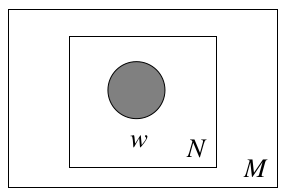
\includegraphics[width=\textwidth]{unigram}
        \caption{Unigram Model}
        \label{fig:uni}
    \end{subfigure}
    \begin{subfigure}[b]{0.3\textwidth}
        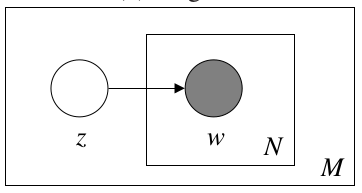
\includegraphics[width=\textwidth]{mixunigram}
        \caption{Mixture of unigrams}
        \label{fig:mix}
    \end{subfigure}
    \begin{subfigure}[b]{0.3\textwidth}
        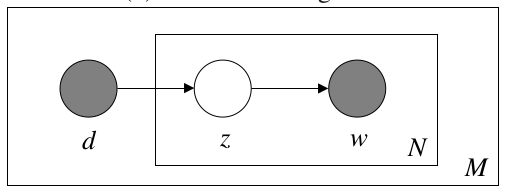
\includegraphics[width=\textwidth]{plsi}
        \caption{pLSI}
        \label{fig:plsi}
    \end{subfigure}
    \caption{Graphical representations for topic models}
\end{figure}


\subsubsection{Mixture of Unigrams}

In the mixture of unigrams, each document has its own multinomial distribution.
These distributions do not represent topics--they are just a document-specific distribution of
words. The generative process draws a parameter $z$ for each document, and then
words are drawn from a multinomial conditioned on $z$. Mathematically, this is
represented by

\[
  p(w) = \sum_z p(z) \prod\limits_{n=1}^N p(w_n | z)
\]

Graphically, this is represented by the process shown in Figure~\ref{fig:mix}

\subsubsection{Probabilistic Latent Semantic Indexing}

pLSI extends the mixture of unigrams model further, by postulating that a
document $d$'s words are independent of the document index given an unobserved
topic, $z$. It is represented graphically by Figure~\ref{fig:plsi}.

\subsubsection{Latent Dirichlet Allocation}
\label{sec:lda}

Latent Dirichlet Allocation extends all of the previous models by assuming that
there is some fixed global parameter which controls the topic distributions of
the documents. There is then a per-topic probability of a word showing up in a
document, which is modified by another global parameter. Graphically, it is
represented by Figure~\ref{fig:ldagraph}.

\begin{figure}
  \centering
  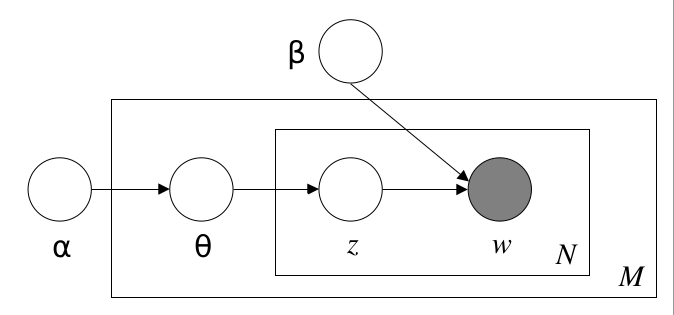
\includegraphics[width=0.7\textwidth]{lda}
  \caption{Graphical Model for LDA}
  \label{fig:ldagraph}
\end{figure}

Algorithimically, the generative process is assumed to draw topic distributions
from a Dirichlet distribution. Then, for each individual document in the corpus,
the following happens:

\begin{enumerate}
\item Choose the document length $N$, either as a fixed parameter or from a Poisson
  distribution.
\item Choose a document topic composition $\theta \sim \text{Dir}(\alpha)$
\item For each of the $N$ words:
  \begin{enumerate}
  \item Choose a topic $z_n \sim \text{Multinomial}(\theta, 1)$
  \item Choose a word $w_n$ from $p(w_n | z_n, \beta_{z_n})$
  \end{enumerate}
\end{enumerate}

As can be seen from Figure~\ref{fig:ldagraph}, this model is significantly more
complicated than any of its predecessors. What it loses in simplicity, however,
it more than makes up for in power. On top of being able to account for a
probabilistic distribution of words in a topic, LDA is additionally posits that
a document can contain multiple topics, and that there is some global
distribution of topics (controlled by $\alpha$) which the topic mixtures come
from.

The question that arises now is this: can we efficiently solve this model? For a
long time, the only available solution method was batch variational inference,
which is very slow when the number of documents and topics is large. Instead, a
more recent invention, stochastic variational inference, can be used to quickly
calculate the posterior distribution.

\subsection{Stochastic Variational Inference}

Variational inference is one technique that can be used when a posterior
distribution is intractable to compute explicitly. By introducing some
parametrized distribution over the hidden variables and minimizing the
difference between the variational distribution and the posterior, we can
approximate the posterior distribution.

Variational inference minimizes the evidence lower bound (ELBO), which is equal
to the negative Kullback-Leibler divergence plus an additive constant.

To derive the ELBO, we assume we have a probability distribution over all
variable in the model (in this example case, $x,z,\beta$), and introduce
a distribution over some hidden variables, $q(z,\beta)$.

\begin{align*}
  \log p(x) &= \log \int  p(x,z,\beta) dz d\beta \\
            &= \log \int p(x,z,\beta) \frac{q(z,\beta)}{q(z,\beta)} dz d\beta\\
            &= \log \left( \bbE_q \left[ \frac{p(x,z,\beta)}{q(z,\beta)} \right] \right)\\
            &\geq \bbE_q[\log p(x,z,\beta)] - \bbE_q[\log q(z,\beta)]\\
            &\triangleq L(q)
\end{align*}

By making appropriate choices for the forms of $q$ and modifying the gradient of
the PDF by the Fisher matrix (which results in the so-called natural gradient),
we can arrive at the general algorithm for stochastic variational inference in
Appendix A.

The specific variational inference algorithm for LDA is provided in
Listing~\ref{lst:svilda}. For ease of understanding, some of the types and sizes
of parameters have been added to the algorithm. The numbers used for dimensions
are as follows: $K$ is the number of topics, $N$ is the number of distinct words
in the document corpus, $D$ is the number of documents, and $M$ is the number of
words in a given document. Superscripts in parenthesis are used to refer to the
time series, while superscripts without parenthesis are used to refer to a
document ID, e.g. $w_n^d$ is the $n$th word in the $d$th document. This differs
slightly from the original notation because, quite frankly, I wouldn't wish the
original notation on my enemies.

In addition, words are represented indicator vectors, that is $w_n^d$ is a vector with $N$
entries, all but one of which are zero. When used as a subscript, it refers to
the nonzero index in the indicator vector, instead of the full vector.

If a matrix-valued variable is subscripted with a single subscript, it
refers to that column of the matrix, e.g. if $X$ is a matrix, $X_i$ is the $i$th
column of $X$.

Alpha and eta ($\alpha,\eta$) are hyperparameters provided by the user. A sane
value is somewhere between 0.1 and 1.

Finally, the variable $\Psi$ is used to refer to the digamma function, which is
equal to the derivative of the log of the gamma function:

\[
  \Psi(x) = \frac{d}{dx} \log \left( \Gamma(x) \right)
\]

\begin{lstlisting}[caption={The SVI-LDA algorithm},label={lst:svilda},
mathescape=true, keywords={}]
Declare $\lambda$: a matrix of size $k \times n$
Set $\rho^{(0)}$ in $[0.5,1)$
while $\lambda$ not converged:
  while $\phi$ and $\gamma$ not converged:
		Sample a document indexed by $d$ randomly from the corpus
		Declare $\gamma^d$: a vector with $K$ elements
		Declare $\phi^d$: a matrix of size $k \times M$

		Initialize $\gamma_k^d = 1$ for $k \in \{1, \dots, K\}$
		For $m \in \{1,  \dots, M\}$: 			(words in document)
			For $k \in {1, \dots, K}$: 			(topics)
				Set $\phi_{m,k}^d \propto \left( \Psi(\gamma_k^d) - \sum_{j=1}^{K}\
             \Psi(\gamma_j^d) \right) -\
             \left( \Psi(\lambda_{k,w_n^d}) - \sum_{j=1}^M \Psi(\lambda_{k,j})\
             \right)$
		
		Set $\gamma^d = \alpha + \sum_m \phi^d_m$
	endwhile

  For $k \in \{1, \dots, K\}$:
		Set intermediate topics $\hat{\lambda}_k = \eta + D \sum_{m=1}^M \phi_{mk}^d
w_{dm}$
	endfor

	Update $\lambda^{(t)} = (1 - \rho^{(t)})\lambda^{(t-1)} + \rho^{(t)}\hat{\lambda}$
  Update $\rho^{(t)}$ by some rule, e.g. Robbins-Munro or Adagrad 
endwhile

\end{lstlisting}

The per-document parameters $\gamma$ and $\phi$ can either be stored during
computation and reused, or the global parameter $\lambda$ can be used to
reconstruct them once it is found, using a procedure similar to that between
lines 5 and 15 in Listing~\ref{lst:svilda}. Once $\phi, \gamma$, and $\lambda$
are known for a particular document and corpus, they can be used to extract
information about the topics in each document and the per-topic distribution of words.

\section{Code \& Results}

Unfortunately, due to time constraints, I was unable to get my SVI running at
scale on a large body of documents. Instead, I created a corpus of 10,000
documents from four topics, with about 250 words per topic, using the generative
algorithm described in Section~\ref{sec:lda}. The code to do this is found
in\texttt{ generative.py}, with the topics found in\texttt{ wordlist1.txt}
through\texttt{ wordlist4.txt}. The results are in the directory\texttt{ testdocs}.
\texttt{lda.py} contains the code for doing a simple LDA analysis on the test
corpus.

\subsection{Speed Results}

While getting the lambdas to converge can be done fairly quickly (in
approximately half an hour), calculating the per-document $\gamma$ and $\phi$
distributions is currently surprisingly expensive. Clearly, this is not code
that will run in any reasonable amount of time on 700,000 documents with 7,000
topics.

I suspect that there are three major performance issues with this code:

\begin{enumerate}
\item Lack of sparsity

  While $\lambda$, $\gamma$, and $\phi$ could reasonably be expected to be
  dense, the individual updates to them might not be: in particular, since
  updates to $\phi$ are proportional to an exponential, if one entry of $\phi$
  were significantly larger than all others, it would be reasonable to expect
  that the update can be approximated as a sparse indicator vector.
\item Lack of algorithm-specific optimizations

  In accordance with the above point, I don't know if it's a valid thing to
  always approximate the $\phi$ update as an indicator vector, or if, in some
  rare cases, there will be two phi entries with almost-identical magnitudes, in
  which case the approximation will break down.

  Another such issue arises with the calculation of $\hat{\lambda}_k$. In the
  naive computation, the elements of $\hat{\lambda}_k$ are iterated over in no
  particular order, trashing cache locality. Would it be possible to sort the
  words in the document first and then iterate over them in-order to improve
  cache locality? Would this make a difference? Without explicitly testing
  tweaks like these, it is difficult to say, and unfortunately, I ran out of
  time for testing.

\item No C++ code

  A lot of computation is deeply nested (e.g. calculating the expectations,
  which requires calling a function, which calls\texttt{ digamma}, which calls
 \texttt{gamma}, which calls some lower level functions...) or heavily reliant
 on tight loops (e.g. the loops over the number of topics to update $\phi$),
 both of which are relatively expensive in Python compared to compiled languages
 like C++. In addition, Eigen offers finer control over sparse linear algebra
 than numpy/scipy do, potentially increasing sparse performance further.
  
\end{enumerate}

\subsection{Qualitative Results}

Unfortunately, due to time constraints, I was unable to get my SVI running at
scale on a large body of documents. Instead, I gathered four wordlists from an
english-language-learner's website that had topics, curated them (to avoid
compound words and words with punctuation), and used the algorithm on page 3 to
generate 10,000 sample documents of 1000 words each. The generative code can be
found in\texttt{ generative.py}, while the topics are found in the
\texttt{wordlist\#.txt} files. The topics contained in each file are listed
below--examples of each can be found in Appendix B.

\begin{itemize}
\item \texttt{wordlist1.txt}: Food and Cooking
\item \texttt{wordlist2.txt}: Tools
\item \texttt{wordlist3.txt}: Halloween
\item \texttt{wordlist4.txt}: Boats and the Ocean
\end{itemize}
 
So how well did LDA do? Figure~\ref{fig:ldatopics} shows samples of the topics generated
by LDA. We can see that the upper-left topic corresponds fairly well to the
Halloween topic, the upper-right to Tools, the lower-left to Food and Cooking,
and the lower-right to some combination of the third and fourth wordlists. This
is not particularly surprising, given that the LDA only looked at about 300
documents before converging. If I had forced it to look at all 10,000 documents
before allowing $\rho^{(t)}$ to decrease, it's very likely that the fourth topic
would have been much more homogeneous.

\begin{figure}
  \centering
  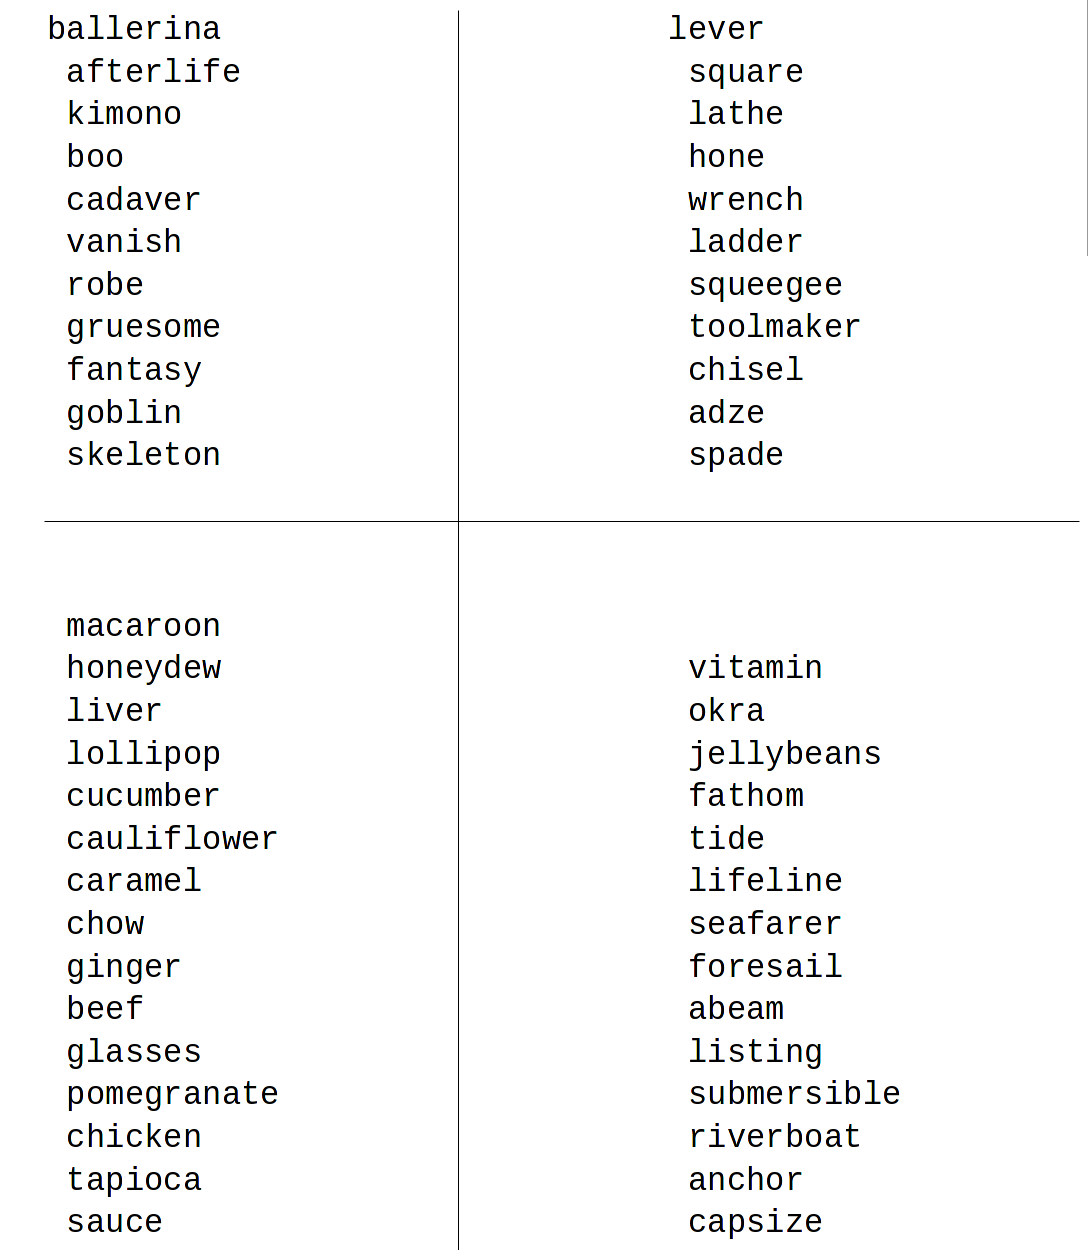
\includegraphics[width=0.5\textwidth]{ldatopics}
  \caption{LDA topic results}
  \label{fig:ldatopics}
\end{figure}

To test this quantitatively, I checked what percent of words in each LDA topic
came from each wordlist. The results are shown in Table~\ref{tab:percents}. 

\begin{table}
  \centering
  \begin{tabular}{l|c|c|c|c|}
    & WL1 & WL2 & WL3 & WL4 \\ \hline \hline
    LDA Topic 1 &  0 & 0 & 1 & 0 \\ \hline
    LDA Topic 2 & 0.039 & 0.961 & 0 & 0.019\\ \hline
    LDA Topic 3 & 0.964 & 0 & 0.035 & 0 \\ \hline
    LDA Topic 4 & 0.571 & 0 & 0 & 0.429
  \end{tabular}
  \caption{Fraction of words from each wordlist in LDA topics.}
  \label{tab:percents}
\end{table}

Clearly, the first 3 topics selected by LDA are fairly pure, and are almost all
from the same topic, with $>96\%$ concentration in one topic. They also agree
with the qualitative assessment above, e.g. LDA Topic 1 comes entirely from
wordlist 3, which is the Halloween topic. The 4th LDA topic suffers from the
issues mentioned above as well, being split almost 50-50 between food and boats.

\section{Conclusion}

\newpage


\section{Appendix A: General Stochastic Variational Inference}

This algorithm is taken near-verbatim out of Hoffman et. al., and so uses some
of their curious notational conventions.

\begin{lstlisting}[mathescape=true, keywords={}]
Initialize $\lambda^{(0)}$ randomly
Set $\rho_t$
repeat until converged:
	Sample a data point $x_i$ from the data set
	Compute its local variational parameter:
			$\phi = \bbE_{\lambda^{(t-1)}}[\eta_g(x_i^{(N)}, z_i^{(N)})]$

	Computer intermediate global parameters:
			$\hat{\lambda} = \bbE_{\phi}[\eta_g(x_i^{(N)}, z_i^{(N)})]$

	Update estimates of lambda:
			$\lambda^{(t)} = (1 - \rho_t) \lambda^{(t-1)}+ \rho_t \hat{\lambda}$

	Update $\rho_t$, e.g. using a Robbins-Munro schedule
end
\end{lstlisting}

\section{Appendix B: Examples of topic words}
\begin{itemize}
\item \texttt{wordlist1.txt}: Food and Cooking
  Examples:
  \begin{itemize}
  \item tamale
  \item lard
  \item sustenance
  \end{itemize}
\item \texttt{wordlist1.txt}: Tools
  Examples:
  \begin{itemize}
  \item adze
  \item scythe
  \item sharpener
  \end{itemize}
\item \texttt{wordlist1.txt}: Halloween
  Examples:
  \begin{itemize}
  \item cauldron
  \item kimono
  \item fog
  \end{itemize}
\item \texttt{wordlist1.txt}: Boats and the Ocean
  Examples:
  \begin{itemize}
  \item warship
  \item pennant
  \item stow
  \end{itemize}
\end{itemize}
\end{document}



\end{document}